\section{Analisi statica}
\note{Quindi iniziamo con la parte \textbf{statica}}

\begin{frame}{Estrazione delle capabilities}
Dato un file eseguibile, andiamo a estrarre le \emph{capabilities} con \textbf{capa}.\\
Usiamo \emph{capa}, strumento open source realizzato da Mandiant.

\note{Dato un file eseguibile, prima di tutto, siamo interessati alle sue capabilities.
Queste sono le possibili azioni che il programma è in grado di compiere. Ad esempio, se può leggere/scrivere file, modificare registri, eseguire operazioni crittografiche, e così via.
\\
Le andiamo ad estrarre usando capa, ossia un tool open source di Mandiant, nonché uno dei più potenti disponibili}

\Pause

\begin{itemize}
    \item Flessibilità con regole custom in YAML
    \note{Ha inoltre il grande vantaggio di permettere l'integrazione di regole YAML che possono essere sia reperite anche da repository pubblici di altre società o ricercatori, senza necessità di modificare il tool ma solo aggiungere file di regole}
    
    \Pause
    \item Successivo parsing dell'output tabellare da testo a JSON machine-readable
    \note{In più, dobbiamo fare il parsing dell'output che fornisce capa, che ovviamente nasce in forma testuale e tabellare, come nella foto, perché è fatto per essere usato interattivamente. Quindi si va ad ottenere un JSON, quindi un formato machine-readable, eseguendo questo parsing.}
\end{itemize}

\begin{figure}
    \centering
    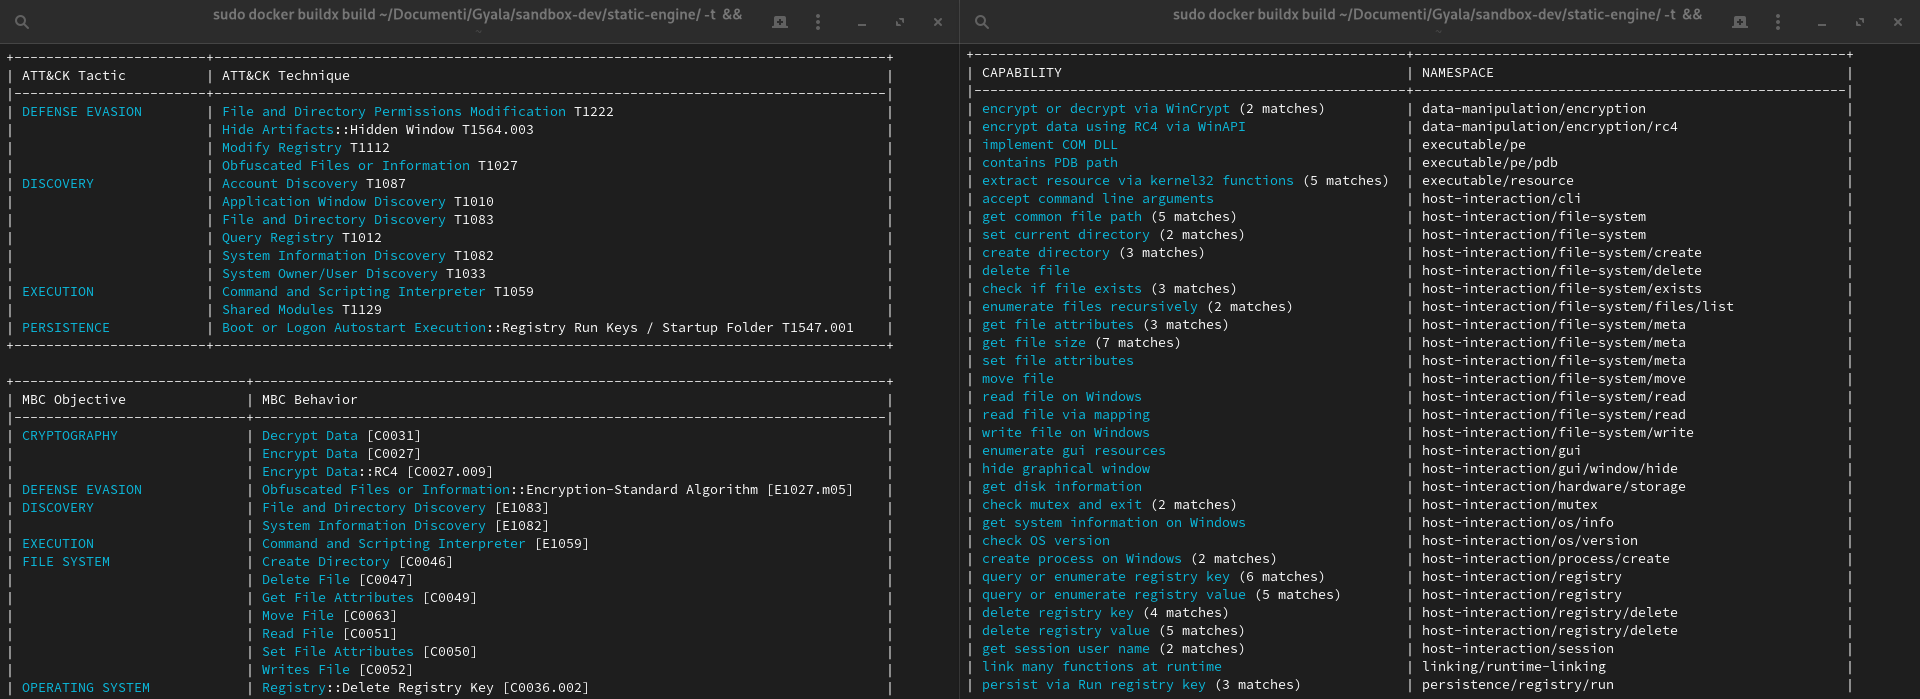
\includegraphics[width=0.75\textwidth]{images/capa_example_invocation.png}
\end{figure}
\end{frame}

% \begin{frame}{Capabilities ottenute}
% \begin{figure}
%     \centering
%     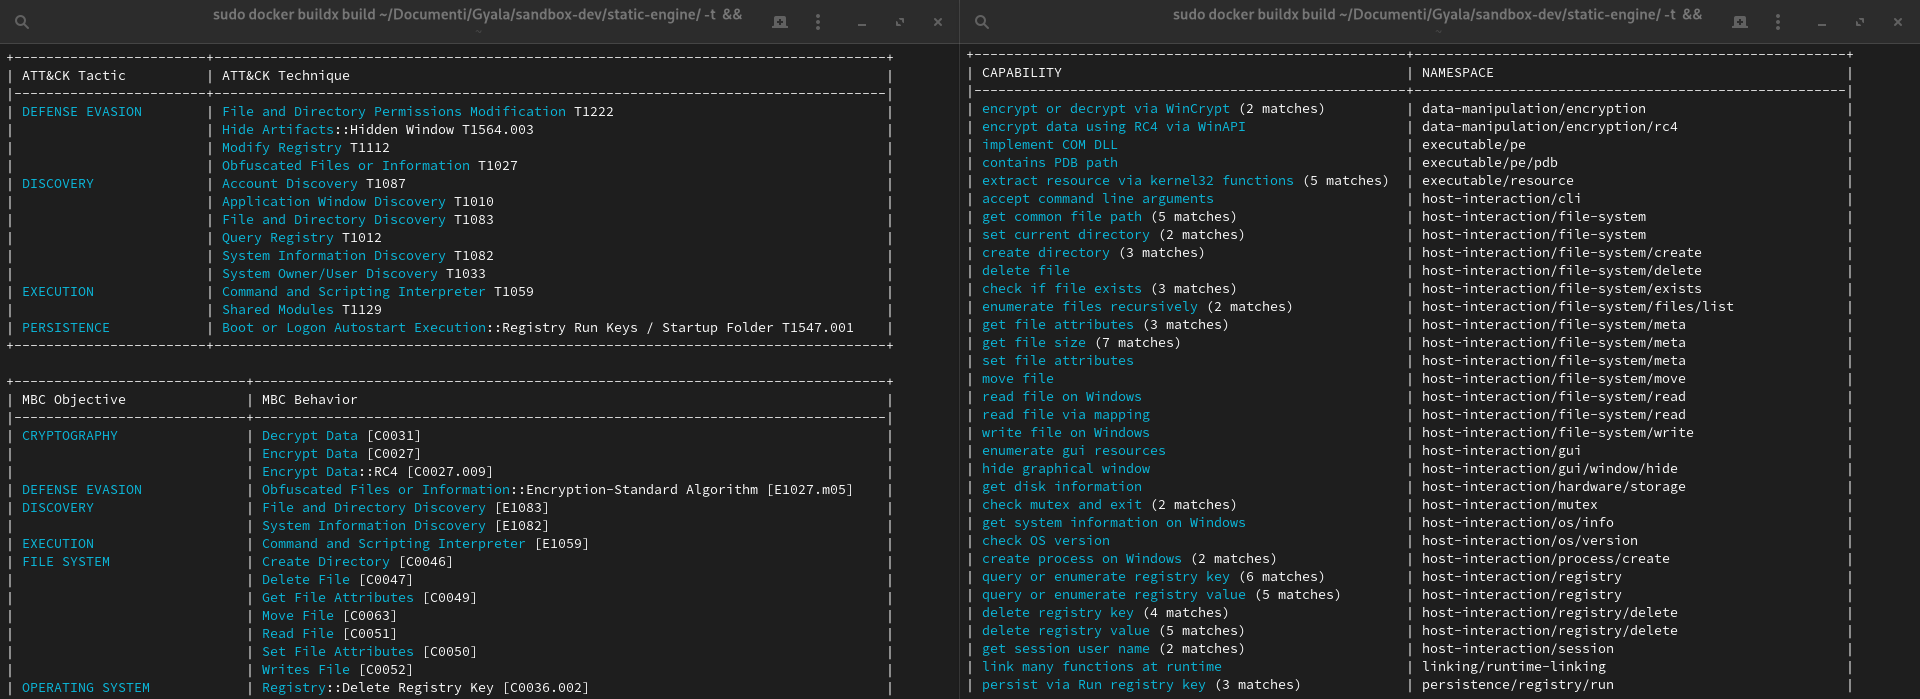
\includegraphics[width=\textwidth]{images/capa_example_invocation.png}
%     \caption{Output restituito da capa}
%     \label{fig:capa_example_invocation}
% \end{figure}
% \end{frame}

% \begin{frame}{Parsing dell'output}
% Non è un formato utilizzabile, bisogna farne il parsing.

% \vfill

% Notiamo la divisione in tabelle, e andiamo a trasformarlo in un JSON.

% Lavoreremo sempre con formato JSON per essere sia human-readable dall'analista che machine-readable da servizi esterni.
% \end{frame}

% \begin{frame}{Output JSON}
% \begin{figure}
%     \centering
%     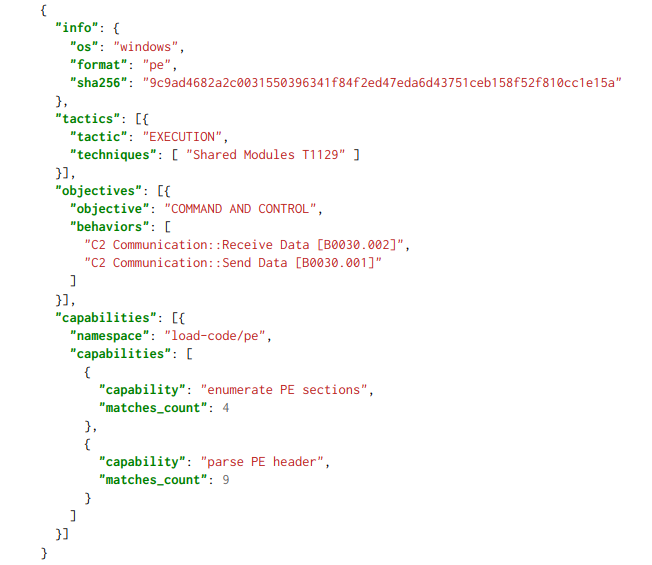
\includegraphics[width=0.57\textwidth]{images/capa_json_output.png}
%     \caption{Output dopo il parsing}
%     \label{fig:capa_json_output}
% \end{figure}
% \end{frame}

\begin{frame}{Casi non supportati}
Capabilities estratte tramire analisi \textbf{statica} del codice.\\
Non sempre funziona (packer, installer, runtime come Visual Basic).
\note{Uno dei più grandi però è la sua fragilità. Infatti l'estrazione delle capabilities avviene tramite un'analisi statica del codice che però non funziona nei casi di eseguibile pacchettizzato, installer o con runtime particolari (es: Visual Basic).
Perchè in questi casi, anche se si tratta di una semplice decompressione a runtime del vero codice dell'eseguibile, resta molto difficile avere risultati che siano affidabili.}

capa terminerà con \textbf{exit code 14}
\vfill

\Pause
\note{
E in questi casi, capa rileva la situazione, terminando con exit code 14.
\begin{itemize}
    \item Può portare a un fallimento dell'intero processo di analisi statica
    \item Ma anche se gestito con try/catch... Crea spreco di risorse (CPU e memoria) per diversi minuti
\end{itemize}
Quindi si va a realizzare tutta una costruzione attorno per renderlo più adatto alle nostre esigenze}

\begin{itemize}
    \item Crash del processo di analisi
    \item Spreco di risorse
\end{itemize}

\end{frame}

\begin{frame}[containsverbatim]{Rilevazione del caso non supportato}
\note{Ma come fa a rilevarlo? All'interno sono presenti delle regole anche per questo scopo.
Il problema però è che la loro esecuzione di default va a richiedere troppo tempo, e vogliamo ridurlo.}
Capa ha regole che rilevano questi casi, ma eseguirle richiede \textbf{troppi minuti.}

\begin{columns}[T]
\begin{column}{0.35\textwidth}
\begin{minted}{yaml}
features:
    - format: pe
    - or:
        - section: UPX0
        - section: UPX1
\end{minted}
\end{column}
\begin{column}{0.63\textwidth}
\begin{minted}{yaml}
features:
    - and:
      - string: /^Inno Setup Setup Data \(/
      - string: /^Inno Setup Messages \(/
\end{minted}
\end{column}
\end{columns}
\vfill
\note{\\\\La nostra rilevazione durerà adesso meno di un secondo, a fronte degli svariati minuti che impiegava il tool, risparmiando in termini di risorse ma di conseguenza anche economicamente. Questo perché andiamo a sfruttare che si tratti solo di rilevare la presenza di particolari sezioni o stringhe, senza avviare l'intero processo di feature extraction}
Dobbiamo creare un \textbf{rilevatore custom} da zero, basandoci sulle regole.
\end{frame}

\begin{frame}{YARA}
Si esegue anche signature-based matching con lo strumento YARA.
\vfill
\begin{figure}
    \centering
    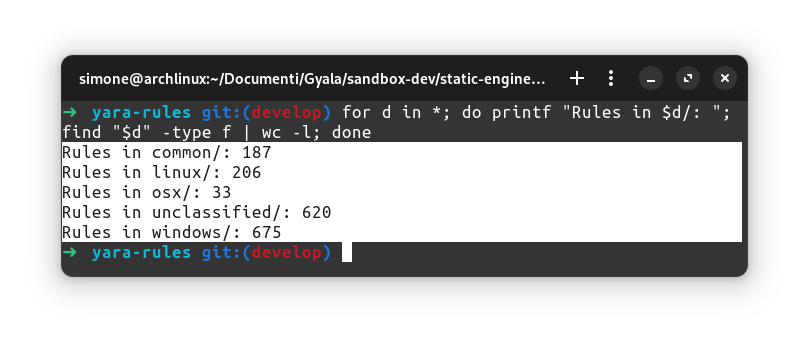
\includegraphics[width=0.9\textwidth]{images/yara_rules_os_separation.png}
    \caption{Divisione delle regole per OS per ottimizzazione}
    \label{fig:yara_rules_os_separation}
\end{figure}

\note{
Successivamente, si è interessati anche ad analisi basate su signature matching, implementate mediante regole YARA.
\\
Queste sono collezionabili da varie realtà della cybersecurity (aziende, ricercatori, ...) \\
oltre a tutte quelle sviluppate internamente
\\
Per ottimizzare l'esecuzione, le regole sono state divise in cartelle ed eseguite solo quando necessario, in base al sistema operativo target, così da omettere quelle inutili
}
\end{frame}

% \begin{frame}{Ulteriori strumenti}
% \begin{itemize}
%     \item \textbf{SSDeep} per fuzzy hashing e correlazione di sample simili tra loro
%     \item \textbf{Detect-It-Easy} e \textbf{ExifTool} estraggono ulteriori metadati dal file in analisi (linker utilizzato, descrizioni, charset, tabella dei simboli, ...)
% \end{itemize}

% \vfill

% Tutti integrati in un \emph{unico flusso di esecuzione} e uniti in uno stesso risultato JSON finale, continuando ad eseguire parsing e trasformazioni di ciò che otteniamo dagli strumenti grezzi
% \end{frame}

\begin{frame}{Flusso di esecuzione}
\begin{figure}
    \centering
    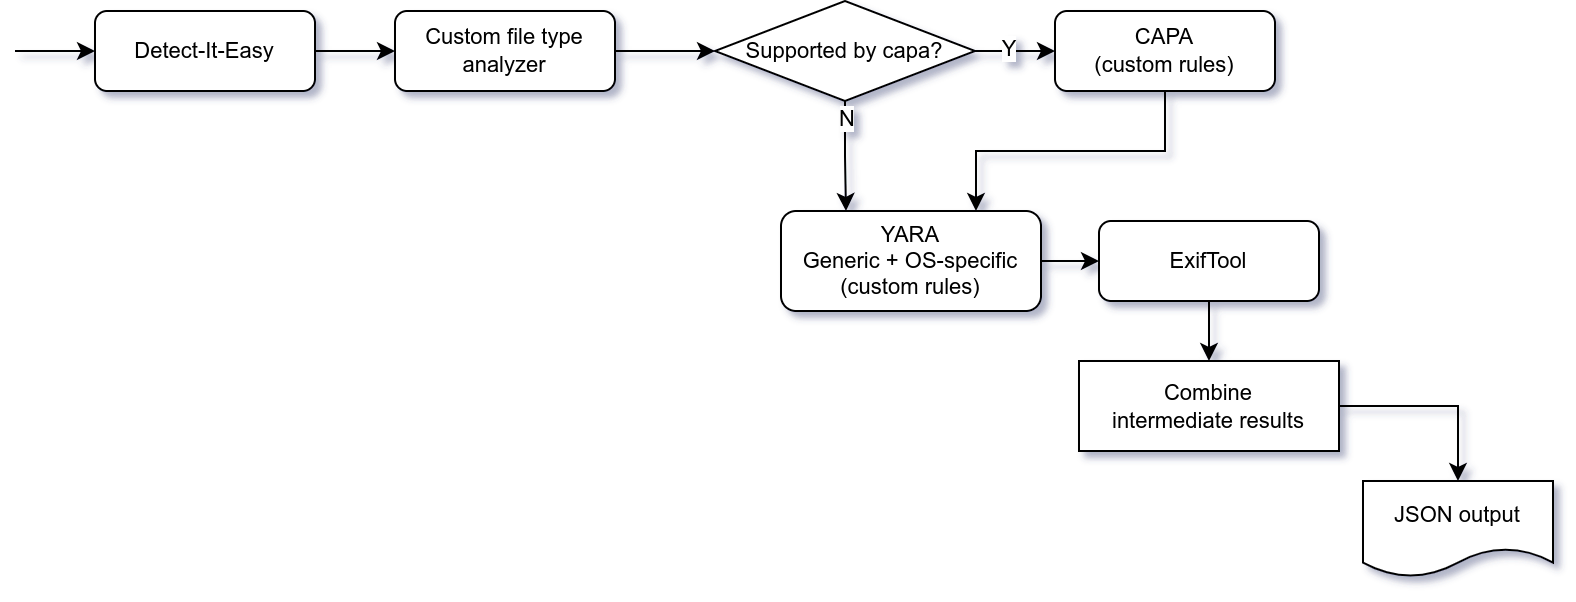
\includegraphics[width=0.9\textwidth]{images/static_run_analysis_internal_tools.png}
\end{figure}


\note{
Nel flusso di esecuzione sono integrate anche altre tecniche minori:
\begin{itemize}
    \item \textbf{SSDeep} per fuzzy hashing e correlazione di sample simili tra loro
    \item \textbf{Detect-It-Easy} e \textbf{ExifTool} estraggono ulteriori metadati dal file in analisi (linker utilizzato, descrizioni, charset, tabella dei simboli, ...)
\end{itemize}
%
Tutti integrati in un \emph{unico flusso di esecuzione} e uniti in uno stesso risultato JSON finale, continuando ad eseguire parsing e trasformazioni di ciò che otteniamo dagli strumenti grezzi
}

\Pause
Errori gestiti tramite handle degli exit-code, garantendo sempre un JSON valido in output

\note{La gestione degli errori avviene tramite handle degli exit-code e restituzione di un JSON contenente il campo \emph{"error"} con un error code tra le stringhe predeterminate}
\end{frame}

% \begin{frame}{Multi-stage build}

% \note{Viene incluso in un container Docker comprensivo di tutte le dipendenze, per massimizzare la portabilità.
% %
% Grazie all'uso intensivo di \textbf{multi-stage build} si è ridotta la sua dimensione finale a $\approx$ 200 MB, partendo da oltre 2 GB se creata in modo naive
% %
% Sfrutta anche la cache per le build seguenti e la parallelizzazione usando \texttt{docker buildx}}

% \begin{figure}
%     \centering
%     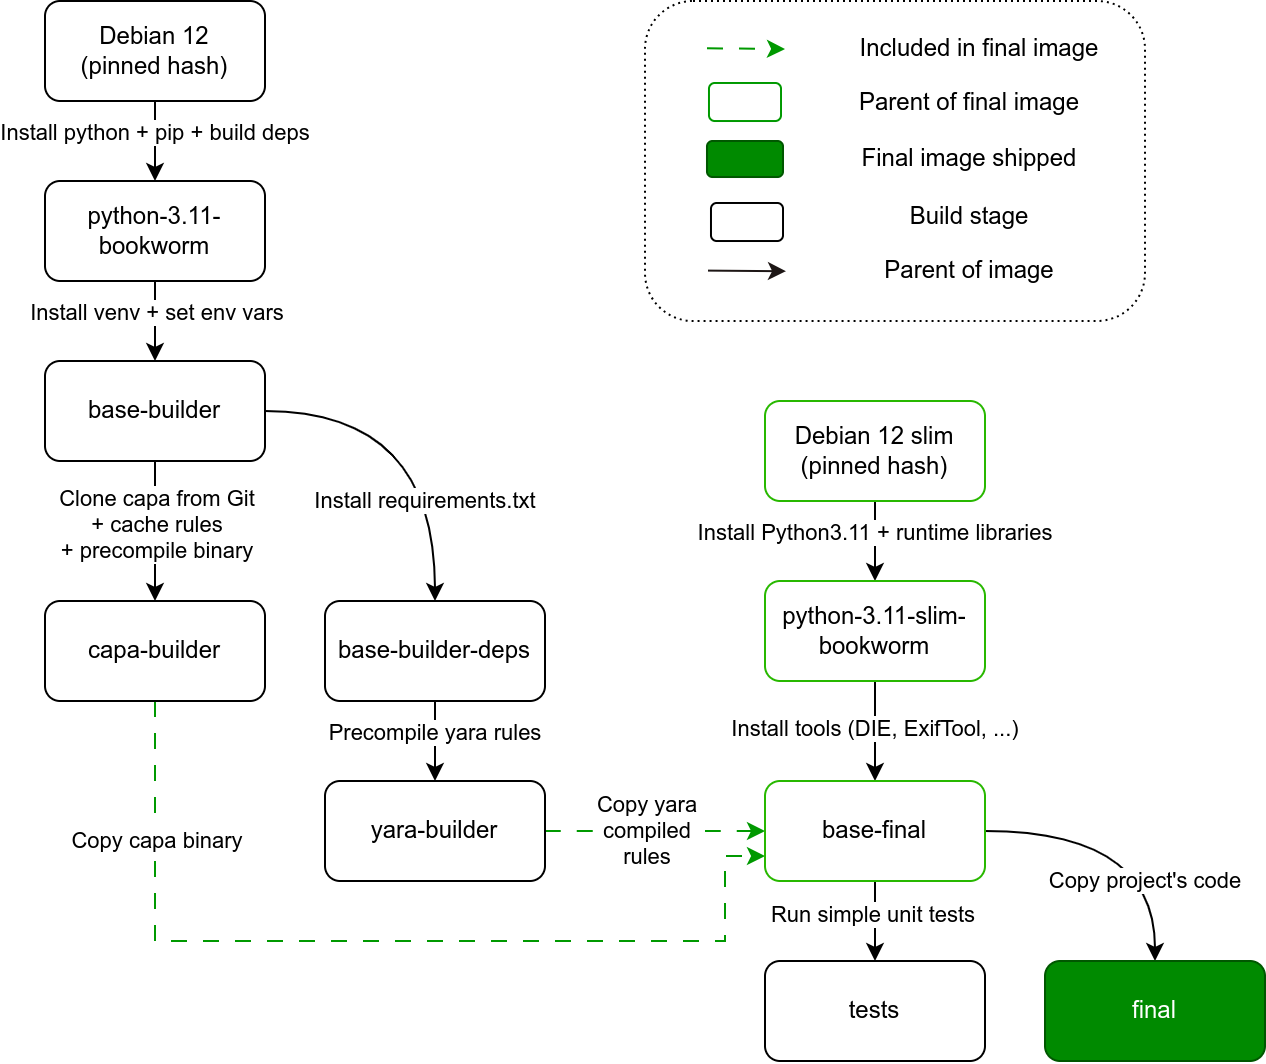
\includegraphics[width=0.6\textwidth]{images/dockerfile.png}
% \end{figure}
% \end{frame}

\begin{frame}{Architettura - deploy su AWS}
\begin{figure}
    \centering
    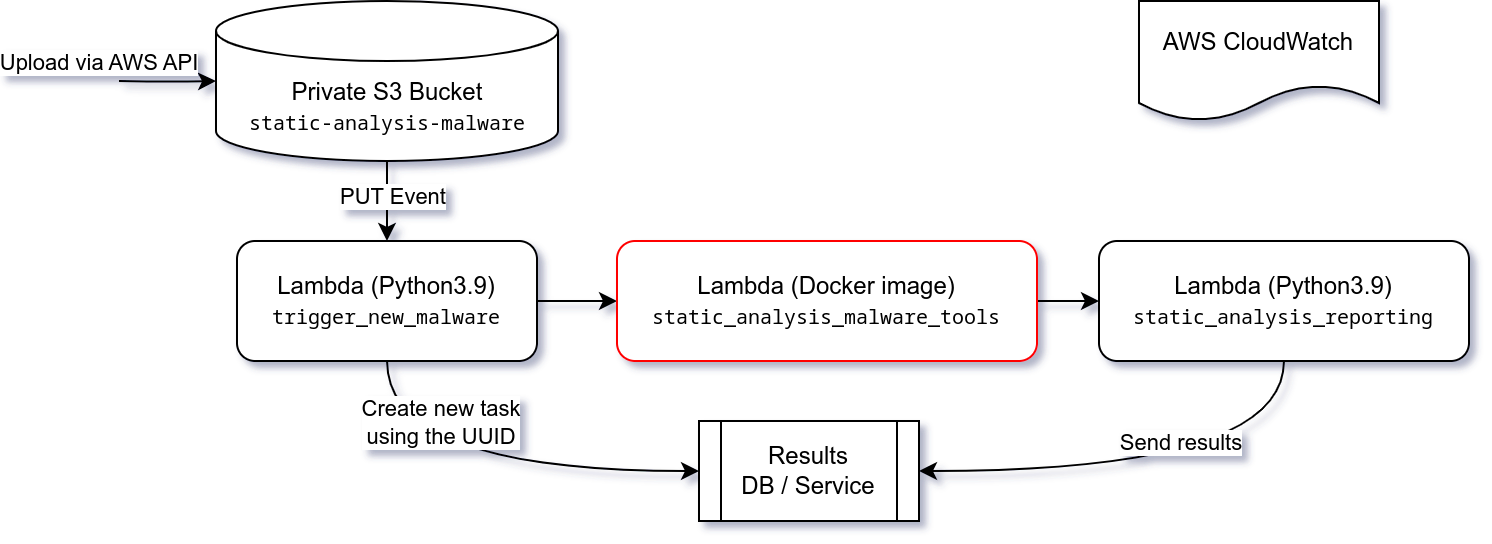
\includegraphics[width=\textwidth]{images/aws_static_lambdas_architecture.png}
\end{figure}
\note{
Una volta fatto il deploy in cloud su AWS, questo è il flusso di esecuzione a più alto livello, dove ciò che abbiamo appena visto è tutto all'interno della Lambda malware\_tools, distribuita come un'immagine Docker.
\\
Dopo un'analisi dei costi e delle caratteristiche di AWS Lambda, EC2 e simili, si è optato per eseguire questa analisi su AWS Lambda. E qui ne vediamo 3 distinte, non una sola.
Questo perché si creano varie Lambda per minimizzare i permessi assegnati dove viene effettivamente analizzato il malware, seguendo il principio del \emph{Least Privilege}
}
\end{frame}

% \begin{frame}{Compressione del risultato}
% Per non usare inutilmente un bucket S3 per salvare i risultati, viene passato il JSON finale da \texttt{static\_analysis\_malware\_tools} a \texttt{static\_analysis\_reporting}.
% \vfill
% AWS limita questo payload a 6MB, spesso viene superato.
% \vfill
% Si è scelto di comprimere il JSON con gzip, poi reso una stringa ASCII usando Base64.
% Se ancora si superano i 6MB si emette un errore, ma è un caso raro o dovuto a regole YARA mal scritte.
% \end{frame}

% \begin{frame}{Compressione del risultato}
% \begin{figure}
%     \centering
%     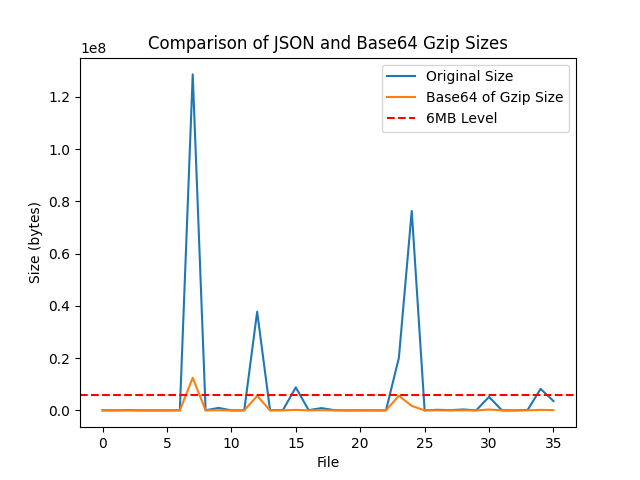
\includegraphics[width=0.5\textwidth]{images/static_analysis_results_size.png}
%     \caption{Differenza tra la dimensione prima e dopo la compressione}
%     \label{fig:static_analysis_results_size}
% \end{figure}
% \end{frame}

\begin{frame}{Pipeline CI/CD}
Viene realizzata anche una pipeline CI/CD per GitLab Runner.
\note{Per automatizzare anche il processo di deploy dello strumento, si è creata una pipeline CI/CD su GitLab che esegue in appositi Runner.\\\\}
\vfill
\note{Così, se si modifica una regola o esegue una modifica, al push del commit Git viene eseguito: 
\textbf{GLI STEP}}
\begin{itemize}
    \item \textbf{build} dell'immagine Docker, usando \emph{multi-stage build} per ridurne la dimensione da 2GB a $\approx$ 200MB
    \item \textbf{test} usando dei file innocui creati per varie architetture, sistemi operativi e casistiche (tradizionali, packed, installer, ...)
    \item \textbf{deploy} dell'immagine su AWS ECR e sulla Lambda in caso di test positivi
\end{itemize}
\end{frame}